\begin{figure}[H] \label{fig:true-cholesky-heatmaps}
\centering
\subfloat[I]{
  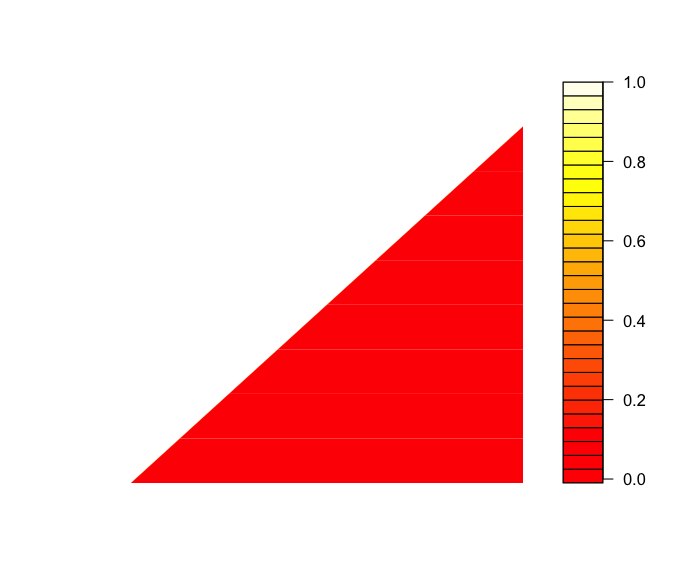
\includegraphics[width = .2\textwidth]{../img/chapter-4/true-cholesky-1-heat-map}
} 
\subfloat[II]{
  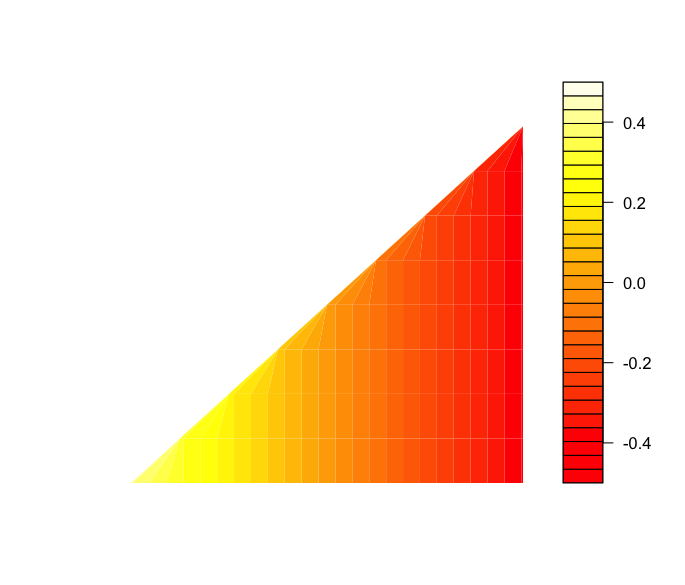
\includegraphics[width = .2\textwidth]{../img/chapter-4/true-cholesky-2-heat-map}
} 
\subfloat[III]{
  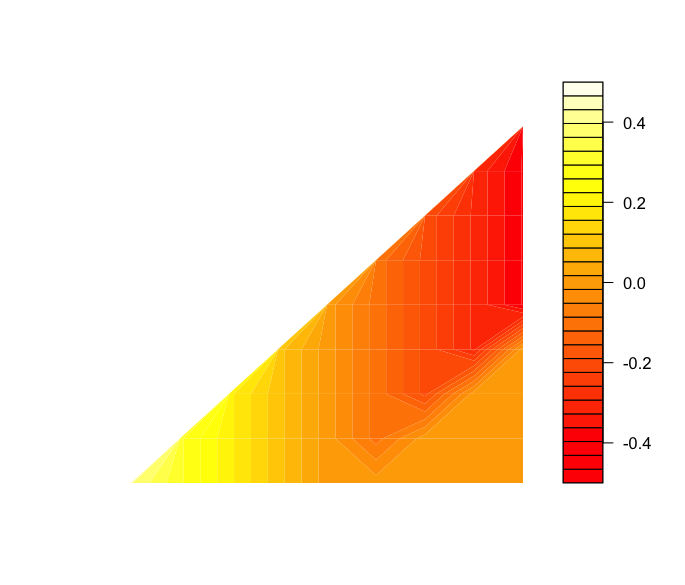
\includegraphics[width = .2\textwidth]{../img/chapter-4/true-cholesky-3-heat-map}
} 
\subfloat[IV]{
   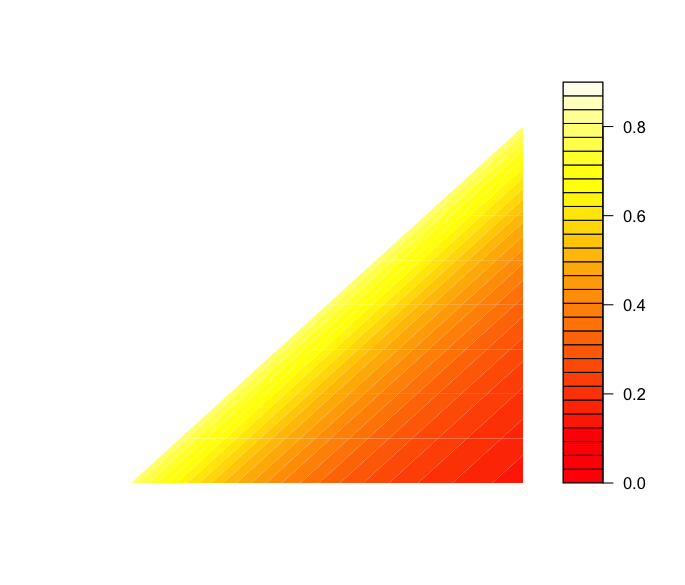
\includegraphics[width = .2\textwidth]{../img/chapter-4/true-cholesky-4-heat-map}
   }
\subfloat[V]{
  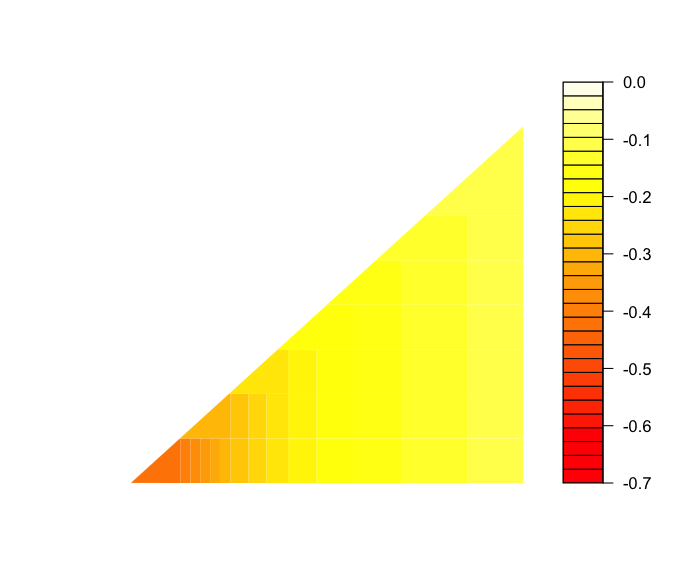
\includegraphics[width = .2\textwidth]{../img/chapter-4/true-cholesky-5-heat-map}
}
\caption{True cholesky surfaces corresponding to Model~\ref{item:cov-type-1} - Model~\ref{item:cov-type-5}}
\end{figure}